\documentclass[final,a4paper,times,3p,onecolumn]{elsarticle}
\usepackage[spanish]{babel}
\usepackage[utf8]{inputenc}
\begin{document}
\begin{frontmatter}
\title{Utilización microbiana de la lignina}
\author[deg]{Eliana Molina Moya}
\ead{elianamm185@gmail.com}
\address[deg]{Universidad de Granada}
\begin{abstract}
En la actualidad se está intentando apostar por el cambio de una economía basada en combustibles fósiles a una basada en biotecnología, sin embargo es una propuesta que está resultando difícil llevar a cabo. A nivel industrial la mayor parte del procesamiento de biomasa utilizan celulosas y hemicelulosas para producir bioetanol y papel. Sin embargo, no existe un bioproceso consolidado para producir compuestos valiosos a partir de la lignina. Por lo general, la lignina se quema para proporcionar calor o permanece como subproducto en diferentes corrientes, afectando negativamente al medio ambiente.  La naturaleza ofrece un arsenal de herramientas biotecnológicas a través de microorganismos para lograr la valorización y/o degradación de la lignina. En esta revisión, se describen algunos informes sobre la utilización microbiana de la lignina para producir compuestos útiles, así como para disminuir su impacto ecológico. \textit{Repositorio https://github.com/elianamm185/proyecto\_final}
\end{abstract}	

\begin{keyword}
Biocatalisis \sep Bioproceso \sep Biorremediación \sep Lignocelulosa \sep Lignina 
\end{keyword}

\end{frontmatter}

\section{Introducción}
Según los últimos cálculos, en 15 años la demanda global de energía va a incrementar en un 50 \% \cite{McCann2015}. En esta situación, y debido al impacto ambiental causado por el uso de combustibles fósiles es indispensable la búsqueda de fuentes de energía alternativas: las fuentes renovables. Desde hace años, la biomasa lignocelulósica se está considerando una buena opción a partir de la cual desarrollar una economía basada en biocombustibles. Sin embargo, hay que tener en cuenta para su uso, que es de naturaleza recalcitrante, es decir,  que las paredes celulares ofrecen resistencia a la descomposición en azúcares monoméricos, una característica que le es concebida por su contenido en lignina. La generación de energía, fuel, productos químicos de construcción, y otros productos fuera de la biomasa lignocelulósica es lo que define el concepto de biorefinería \cite{Maity2015}. La producción de bioetanol y papel a partir de la biomasa de las plantas solo comprende el uso neto de la celulosa y hemicelulosa, mientras que la lignina normalmente se quema para producir calor o esta se queda como producto de los efluentes industriales causando un daño medio ambiental a causa de su naturaleza ácida. La naturaleza por sí misma ofrece múltiples vías de degradación de la lignina a través de una gran variedad de microorganismos. Algunos ejemplos se muestran en la Figura\,\ref{Fig1}.

\begin{figure}
	\centering
	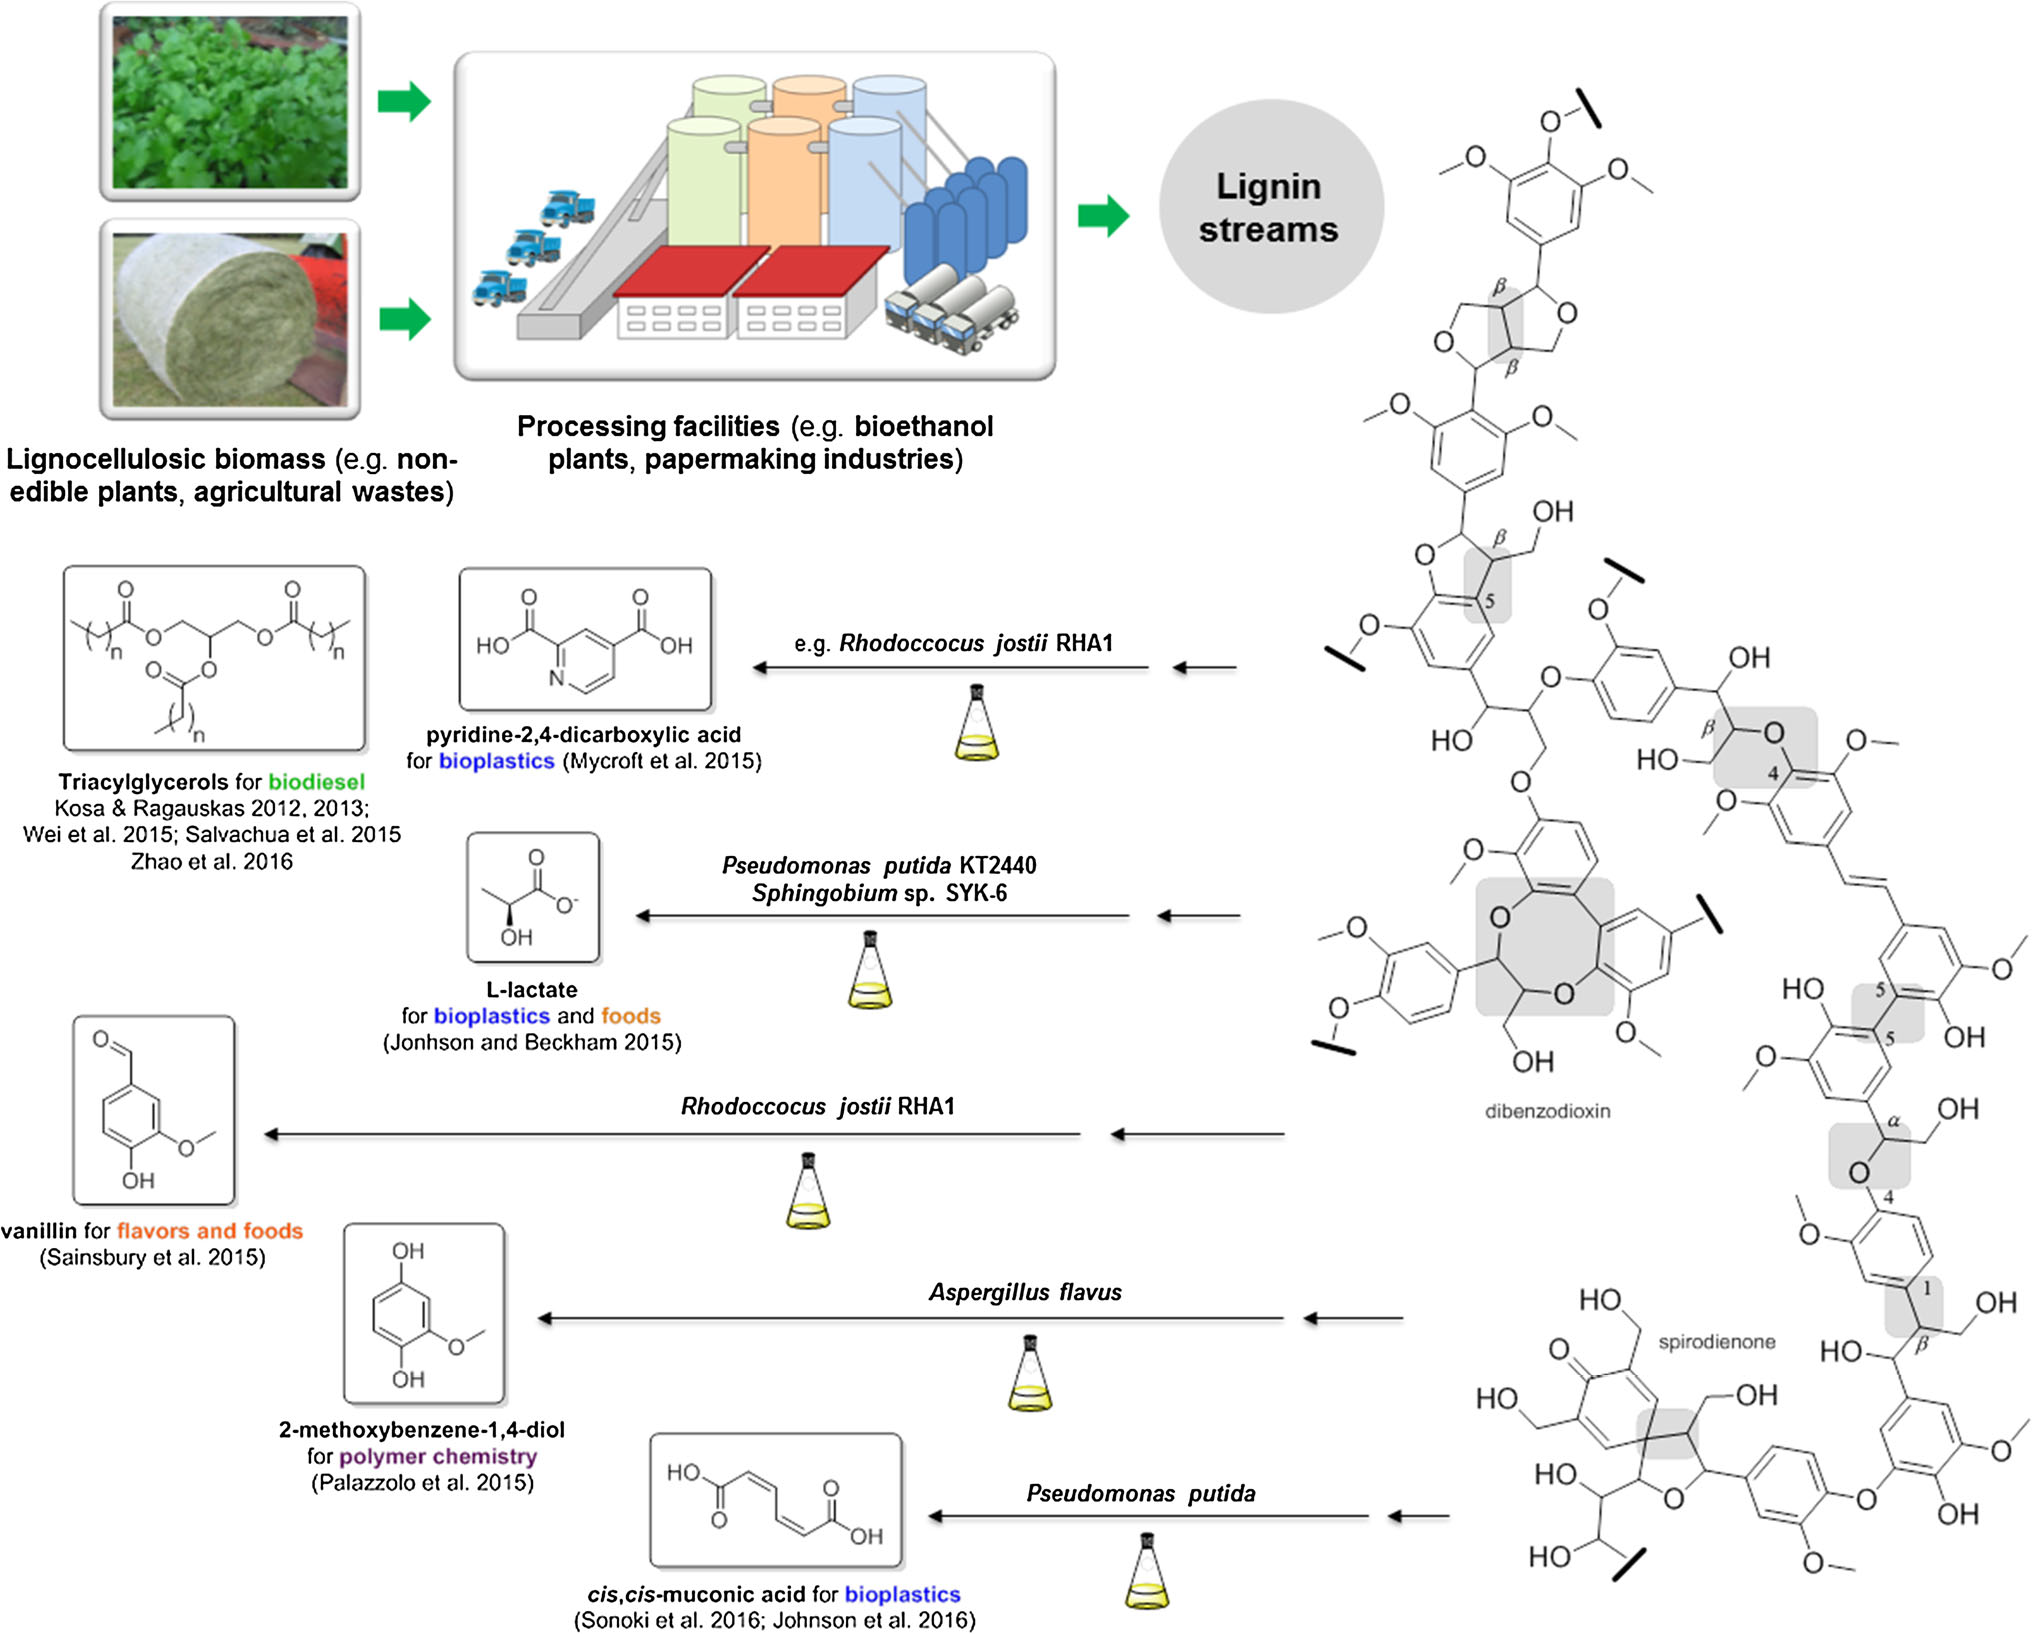
\includegraphics[width=10cm]{figura1.png}
	\caption{Estrategias de valorización de la lignina}
	\label{Fig1}
\end{figure}
\section{Aislamiento y uso de hongos para la degradación de la lignina}

Los hongos de la podredumbre de la madera son importantes herramientas biotecnológicas para aprovechar la biomasa de las plantas debido a su habilidad de secretar un set de enzimas lignocelulolíticas en grandes cantidades. Estos incluyen especies del filo Ascomycota y Basidiomycota, que son hongos de la podredumbre parda  y blanca de la madera respectivamente \cite{dashtban2010}. Desde una perspectiva de producción, principalmente son los hongos de la podredumbre parda los que se usan para fermentar los polisacáridos de la biomasa vegetal, pero estos no realizan la degradación de la lignina, o lo hacen muy poco. Por el contrario, los hongos de la podredumbre blanca de la madera son muy eficientes en la degradación de la lignina y algunos presentan una alta selectividad, por lo que dejan la celulosa y hemicelulosa intactas \cite{Makela2014}. Las enzimas comprenden hemo peroxidasas – como la lignina, manganeso o versátil peroxidasa- y la lacasa. También se necesitan enzimas accesorias tales como oxidasas que generan peróxido de hidrógeno. 
De forma alternativa, los hongos de la podredumbre parda emplean un mecanismo no enzimático como primera etapa de degradación lignocelulósica para producir radicales hidroxilo a través de las reacciones de Fenton, y así permiten la penetración de enzimas de sacarificación \cite{Arantes2012}. La función final de los hongos en la producción del etanol a partir de la biomasa lignocelulósica se ha descrito ampliamente por una serie de autores en los últimos años, y es en definitiva, permitir el acceso a los azúcares fermentables (como ocurre en el proceso de fabricación del papel durante la etapa de blanqueamiento).
 
Hay una variedad de procesos que comprenden el uso de los hongos para reducir el contenido de la lignina, como es por ejemplo, la mejora de la calidad nutritiva de los rumiantes. En un caso se ensayó el cultivo de \textit{Gloephyllum trabeum} KU-41 con la sobreexpresión de una lacasa endógena que producía un aumento de un 45 \% (respecto a la cepa silvestre) en la producción de etanol, a partir de la madera del cedro japonés \cite{Arimoto2015}. Otro estudio que podemos mencionar es el de Chang et al. (2012) en el que encontraron una cepa de Fusarium moniliforme con alto poder de deslignificación en la paja de arroz pero casi inactivo en la fracción de holocelulosa \cite{Chang2012}. Esta cepa representaba una buena elección para preparar materia prima de rumiantes. Por último Liang et al. (2010) determinaron que la adición de pequeñas cantidades de biosurfactante dirhamnolipídico aumentaba la actividad ligninolítica del hongo de la podredumbre blanca \textit{Phanerochaete chrysosporium} en la paja de arroz \cite{Liang2010}.

\section{Descubrimiento y aplicación de bacterias degradadoras de lignina}
Algunas bacterias también se han descrito por su habilidad de romper la lignina. La mayoría de las bacterias que muestran actividad ligninolítica comprenden el filo Proteobacteria, Actinobacteria, Firmicutes, y en menos extensión, Cyanobacteria, Bacteriodetes y Spirochaetes \cite{Tian2014}. Gracias a la ingeniería genética y a la expresión de las proteínas fúngicas, el uso de las bacterias está teniendo gran atracción, ya que es más fácil trabajar con ellas. La utilización de microorganismos o de las enzimas producidas por estos, combinado con la aplicación de químicos, puede permitir el desarrollo de diferentes estrategias que entran dentro del concepto biorefinería. Además, hay nuevos avances que están permitiendo manipular la plasticidad biosintética de la lignina en las plantas, para así facilitar su degradación.

Como se ha dicho antes, para que el concepto de biorefinería sea fascible económicamente, es necesario utilizar toda la biomasa lignocelulósica, sin descartar la lignina, la cual puede servir para preparar químicos valiosos. En recientes estudios, se ha tratado de buscar los diferentes componentes valiosos y renovables que se pueden producir a partir de la lignina. Chen et al. (2012) cultivaron Comamonas sp. de fluidos de hojas de bambú capaces de crecer en muchos componentes derivados de la lignina y degradaban más de 0,9 g/L de lignina kraft después de 7 días \cite{Chen2012}. Paliwal et al. (2015) aislaron dos cepas bacterianas, \textit{Bacillus megaterium} ETLB-1 y \textit{Pseudomonas plecoglossicida} ETLB-3, del suelo contaminado con los efluentes de la fábrica del papel y resultaba que estos eran capaces de reducir el contenido de la lignina en los licores negros más de 0,8 g/L en 7 días cuando se co-inmobiliza en cubos de mazorca de maíz \cite{Paliwal2014}. Otro estudio interesante fue el realizado por Yang et al. donde encontraron dos especies de Streptomyces procedentes de suelos forestales, que degradaban más de 1,1 g/L de lignina alkali en 12 días cuando se cocultivaba con el hongo de la podredumbre blanca \textit{Pleurotus ostreatus} \cite{Yang2012}. 

\renewcommand{\listtablename}{Índice de tablas}
\renewcommand{\tablename}{Tabla}
\begin{table}[h]
	\centering
	\caption{Biodegradación de lignina por acción de hongos y bacterias}
	\label{tabla1}
	\begin{tabular}{|c|c|c|}
		\hline  \textbf{Fuente de lignina} & \textbf{Microorganismo} & \textbf{Aplicación} \\
		\hline  Cedro japonés &  \textit{Gloeophyllum trabeum} & Producción de bioetanol\\
		\hline  Arroz  &  \textit{Fusarium moniliforme} & Producción de comida para rumiantes \\
		\hline  Arroz  &  \textit{Phanerochate chrysosporium} &  Biorremediación\\
		\hline  Lignina alkali & \textit{Streptomyces} spp. & Biorremediación\\
		\hline  Licor negro & \textit{Bacillus megaterium} & Biorremediación\\
		\hline Lignina kraft & \textit{Comamonas} sp. & Biorremediación\\
		\hline
	\end{tabular}
	
\end{table}

\section{Consideraciones futuras}
Actualmente, existen múltiples posibles formas de utilización de la lignina disponible, algunas de las cuales se mencionan y están recogidas en la Tabla\, \ref{tabla1}. No obstante, para que estos procedimientos se adopten en  la industria, la viabilidad económica debe ser evaluada y garantizada. En esta situación, con la ayuda de la biología e ingeniería metabólica, deben diseñarse bioprocesos costo-efectivos. Tanto las técnicas tradicionales como las técnicas avanzadas de detección son todavía necesarias, considerando que una porción inmensurable del microbioma de la tierra sigue siendo desconocido.

Por otra parte, los microorganismos ligninolíticos conocidos no han sido estudiados completamente aún. Por lo tanto, los informes emergentes de la metagenómica ambiental, así como las próximas tecnologías de generación de secuencias, serían de gran ayuda. Además, el concepto de diseñador de lignina puede desarrollarse aún más para facilitar la degradación y la valorización de la lignina en la práctica. Por último, decir que las estrategias de utilización de la lignina aún son muy ineficaces. 

Por todas estas razones, es necesario animar a los científicos para que continúen profundizando en este tema, y a las industrias para que apuesten por incluir bioprocesos, como es el que se trata aquí: la obtención de productos de interés a partir de la degradación de lignina.

\bibliography{bibproyecto.bib} 
\bibliographystyle{plain}

\end{document}

		
		